%% Submissions for peer-review must enable line-numbering
%% using the lineno option in the \documentclass command.
%%
%% Preprints and camera-ready submissions do not need
%% line numbers, and should have this option removed.
%%
%% Please note that the line numbering option requires
%% version 1.1 or newer of the wlpeerj.cls file, and
%% the corresponding author info requires v1.2

\documentclass[fleqn,10pt]{wlpeerj} % for preprint submissions

% ZNK -- Adding headers for pandoc

\setlength{\emergencystretch}{3em}
\usepackage[unicode=true]{hyperref}


% tightlist command for lists without linebreak
\providecommand{\tightlist}{%
  \setlength{\itemsep}{0pt}\setlength{\parskip}{0pt}}

% From pandoc table feature
\usepackage{longtable,booktabs,array}
\usepackage{calc} % for calculating minipage widths
% Correct order of tables after \paragraph or \subparagraph
\usepackage{etoolbox}
\makeatletter
\patchcmd\longtable{\par}{\if@noskipsec\mbox{}\fi\par}{}{}
\makeatother
% Allow footnotes in longtable head/foot
\IfFileExists{footnotehyper.sty}{\usepackage{footnotehyper}}{\usepackage{footnote}}
\makesavenoteenv{longtable}

% Pandoc citation processing
\newlength{\cslhangindent}
\setlength{\cslhangindent}{1.5em}
\newlength{\csllabelwidth}
\setlength{\csllabelwidth}{3em}
\newlength{\cslentryspacingunit} % times entry-spacing
\setlength{\cslentryspacingunit}{\parskip}
% for Pandoc 2.8 to 2.10.1
\newenvironment{cslreferences}%
  {}%
  {\par}
% For Pandoc 2.11+
\newenvironment{CSLReferences}[2] % #1 hanging-ident, #2 entry spacing
 {% don't indent paragraphs
  \setlength{\parindent}{0pt}
  % turn on hanging indent if param 1 is 1
  \ifodd #1
  \let\oldpar\par
  \def\par{\hangindent=\cslhangindent\oldpar}
  \fi
  % set entry spacing
  \setlength{\parskip}{#2\cslentryspacingunit}
 }%
 {}
\usepackage{calc}
\newcommand{\CSLBlock}[1]{#1\hfill\break}
\newcommand{\CSLLeftMargin}[1]{\parbox[t]{\csllabelwidth}{#1}}
\newcommand{\CSLRightInline}[1]{\parbox[t]{\linewidth - \csllabelwidth}{#1}\break}
\newcommand{\CSLIndent}[1]{\hspace{\cslhangindent}#1}

\usepackage{lipsum} \usepackage{placeins} \usepackage[htt]{hyphenat} \usepackage{booktabs} \usepackage{microtype}

\usepackage{flafter}
\usepackage{float}
\usepackage{booktabs}
\usepackage{longtable}
\usepackage{array}
\usepackage{multirow}
\usepackage{wrapfig}
\usepackage{colortbl}
\usepackage{pdflscape}
\usepackage{tabu}
\usepackage{threeparttable}
\usepackage{threeparttablex}
\usepackage[normalem]{ulem}
\usepackage{makecell}
\usepackage{xcolor}

\title{Bias in estimated short sprint profiles using timing gates due to the flying start: simulation study and proposed solutions}

\author[1]{Mladen Jovanović}

\corrauthor[1]{Mladen Jovanović}{\href{mailto:coach.mladen.jovanovic@gmail.com}{\nolinkurl{coach.mladen.jovanovic@gmail.com}}}

\affil[1]{Faculty of Sport and Physical Education, University of Belgrade, Serbia}


%
% \author[1]{First Author}
% \author[2]{Second Author}
% \affil[1]{Address of first author}
% \affil[2]{Address of second author}
% \corrauthor[1]{First Author}{f.author@email.com}

% 

\begin{abstract}
Short sprints have been modeled using the mono-exponential equation that involves two parameters: (1) maximum sprinting speed (MSS) and (2) relative acceleration (TAU), most often performed using the timing gates. I have named this the \emph{No correction} model. Unfortunately, due to the often utilized flying start, a bias is introduced when estimating parameters. In this paper, I have (1) proposed two additional models (\emph{Estimated TC} and \emph{Estimated FD}) that aim to correct this bias, and (2) provided a theoretical simulation study that provides model performances in estimating parameters. In conclusion, both \emph{Estimated TC} and \emph{Estimated FD} models provided more precise parameter estimates, but surprisingly, the \emph{No correction} model provided better estimates of some parameter changes.
% Dummy abstract text. Dummy abstract text. Dummy abstract text. Dummy abstract text. Dummy abstract text. Dummy abstract text. Dummy abstract text. Dummy abstract text. Dummy abstract text. Dummy abstract text. Dummy abstract text.
\end{abstract}

\begin{document}



\flushbottom
\maketitle
\thispagestyle{empty}

\hypertarget{introduction}{%
\section{Introduction}\label{introduction}}

Sprint speed is one of the most distinctive and admired physical characteristics in sports. In the majority of team sports (e.g., soccer, field hockey, handball, etc.), short sprints are defined as maximal sprinting from a standstill across a distance that does not result in deceleration at the finish. Peak anaerobic power is reached during the first few seconds (\textless5 \(s\)) of maximal efforts (\protect\hyperlink{ref-mangineSpeedForcePower2014}{Mangine et al., 2014}), however the capacity to attain maximal sprint speed is athlete- and sport-specific. For instance, track and field sprinters are trained to achieve maximal speed later in a race (i.e., 50-60 \(m\)) (\protect\hyperlink{ref-ward-smithEnergyConversionStrategies2001}{Ward-Smith, 2001}), whereas team sport athletes have sport-specific attributes and reach maximal speed much earlier (i.e., 30-40 \(m\)) (\protect\hyperlink{ref-brownAssessmentLinearSprinting2004}{Brown, Vescovi \& Vanheest, 2004}). The evaluation of short sprint performance is frequently included in a battery of fitness tests for a wide variety of sports, regardless of the kinematic differences between athletes.

The use of force plates is regarded as the gold standard for analyzing the mechanical features of sprinting; nevertheless collecting the profile of a whole sprint presents practical and cost problems (\protect\hyperlink{ref-samozinoSimpleMethodMeasuring2016}{Samozino et al., 2016}; \protect\hyperlink{ref-morinSimpleMethodComputing2019}{Morin et al., 2019}). Radar and laser technology are frequently utilized laboratory-grade methods (\protect\hyperlink{ref-buchheitMechanicalDeterminantsAcceleration2014}{Buchheit et al., 2014}; \protect\hyperlink{ref-jimenez-reyesRelationshipVerticalHorizontal2018}{Jiménez-Reyes et al., 2018}; \protect\hyperlink{ref-marcote-pequenoAssociationForceVelocity2019}{Marcote-Pequeño et al., 2019}; \protect\hyperlink{ref-edwardsSprintAccelerationCharacteristics2020}{Edwards et al., 2020}) that are typically unavailable to sports practitioners. Timing gates are unquestionably the most prevalent method available for evaluating sprint performance. Multiple gates are frequently placed at different distances to capture split times (e.g., 10, 20, 30, and 40 \(m\)), which can now be incorporated into the method for determining sprint mechanical properties (\protect\hyperlink{ref-samozinoSimpleMethodMeasuring2016}{Samozino et al., 2016}; \protect\hyperlink{ref-morinSimpleMethodComputing2019}{Morin et al., 2019}). Practitioners can utilize the outcomes to explain individual differences, quantify the effects of training interventions, and gain a better knowledge of the limiting variables of performance, which is an advantage of this method.

\hypertarget{mathematical-model}{%
\subsection{Mathematical model}\label{mathematical-model}}

The mono-exponential equation \eqref{eq:velocity-time} has been used to model short sprints. It was first proposed by Furusawa, Hill \& Parkinson (\protect\hyperlink{ref-doi:10.1098ux2frspb.1927.0035}{1927}) and made more popular by Clark et al. (\protect\hyperlink{ref-clarkNFLCombine40Yard2017}{2017}) and Samozino et al. (\protect\hyperlink{ref-samozinoSimpleMethodMeasuring2016}{2016}). Equation \eqref{eq:velocity-time} is the function for instantaneous horizontal velocity \(v\) given time \(t\) and two model parameters.

\begin{equation}
  v(t) = MSS \times (1 - e^{-\frac{t}{TAU}}) \label{eq:velocity-time}
\end{equation}

\emph{Maximum sprinting speed} (MSS; expressed in \(ms-1\)) and \emph{relative acceleration} (TAU; expressed in \(s\)) are the parameters of the equation \eqref{eq:velocity-time}. TAU represents the ratio of MSS to initial acceleration (MAC; \emph{maximal acceleration}, expressed in \(ms-2\)) \eqref{eq:maximal-acceleration}. Note that TAU, given the equation \eqref{eq:velocity-time}, is the time required to reach a velocity equal to 63.2\% of MSS.

\begin{equation}
  MAC = \frac{MSS}{TAU}\label{eq:maximal-acceleration}
\end{equation}

Although TAU is utilized in the equations and afterward estimated, I prefer to use and report MAC because it is simpler to understand, especially for practitioners and coaches.

By deriving the equation \eqref{eq:velocity-time}, we may obtain the equation \eqref{eq:acceleration-time} for horizontal acceleration.

\begin{equation}
  a(t) = \frac{MSS}{TAU} \times e^{-\frac{t}{TAU}}  \label{eq:acceleration-time}
\end{equation}

By integrating equation \eqref{eq:velocity-time}, we get the equation for distance covered \eqref{eq:distance-time}.

\begin{equation}
  d(t) = MSS \times (t + TAU \times e^{-\frac{t}{TAU}}) - MSS \times TAU  \label{eq:distance-time}
\end{equation}

\hypertarget{model-parameters-estimation-using-timing-gates-split-times}{%
\subsection{Model parameters estimation using timing gates split times}\label{model-parameters-estimation-using-timing-gates-split-times}}

Table \ref{tab:example-split-times} contains sample split times measured during 40 m sprint performance using timing gates positioned at 5, 10, 20, 30, and 40 m.



\begin{table}

\caption{\label{tab:example-split-times}Sample split times measured during 40 m sprint performance using timing gates positioned at 5, 10, 20, 30, and 40 m.}
\centering
\begin{tabular}[t]{rr}
\toprule
Distance (m) & Split time (s)\\
\midrule
5 & 1.34\\
10 & 2.06\\
20 & 3.29\\
30 & 4.44\\
40 & 5.56\\
\bottomrule
\end{tabular}
\end{table}

To estimate model parameters using split times, distance is a \emph{predictor} and time is the \emph{outcome} variable; hence, equation \eqref{eq:distance-time} takes the form of the equation \eqref{eq:time-distance}.

\begin{equation}
  t(d) = TAU \times W(-e^{\frac{-d}{MSS \times TAU}} - 1) + \frac{d}{MSS} + TAU \label{eq:time-distance}
\end{equation}

\(W\) in equation \eqref{eq:time-distance} represents Lambert's W function (\protect\hyperlink{ref-R-LambertW}{Goerg, 2022}). Equation \eqref{eq:distance-time}, in which the time is the predictor and distance is the outcome variable, is commonly employed in research (\protect\hyperlink{ref-morinSpreadsheetSprintAcceleration2017}{Morin, 2017}; \protect\hyperlink{ref-morinSpreadsheetSprintAcceleration2019}{Morin \& Samozino, 2019}; \protect\hyperlink{ref-stenrothSpreadsheetSprintAcceleration2020}{Stenroth \& Vartiainen, 2020}), This method should be avoided since reversing the predictor and outcome variables in a regression model may create biased estimated parameters (\protect\hyperlink{ref-motulskyIntuitiveBiostatisticsNonmathematical2018}{Motulsky, 2018, p. 341}). This bias may not be practically significant for profiling short sprints, but it is a statistically flawed practice and should be avoided. It is thus preferable to utilize statistically correct equation \eqref{eq:time-distance} to estimate model MSS and TAU.

Estimating MSS and TAU parameters using equation \eqref{eq:time-distance} as model definition is performed using \emph{non-linear least squares regression}. To the best of my knowledge, scientist, researchers, and coaches have been performing short sprints modeling using the built-in solver function of Microsoft Excel (Microsoft Corporation, Redmond, Washington, United States) (\protect\hyperlink{ref-samozinoSimpleMethodMeasuring2016}{Samozino et al., 2016}; \protect\hyperlink{ref-clarkNFLCombine40Yard2017}{Clark et al., 2017}; \protect\hyperlink{ref-morinSpreadsheetSprintAcceleration2017}{Morin, 2017}; \protect\hyperlink{ref-morinSpreadsheetSprintAcceleration2019}{Morin \& Samozino, 2019}; \protect\hyperlink{ref-morinSimpleMethodComputing2019}{Morin et al., 2019}; \protect\hyperlink{ref-stenrothForcevelocityProfilingIce2020}{Stenroth, Vartiainen \& Karjalainen, 2020}; \protect\hyperlink{ref-stenrothSpreadsheetSprintAcceleration2020}{Stenroth \& Vartiainen, 2020}). These, and additional functionalities, have been recently implemented in the open-source \textbf{\{shorts\}} package (\protect\hyperlink{ref-jovanovicShortsPackageModeling2020}{Jovanović \& Vescovi, 2020}; \protect\hyperlink{ref-vescoviSprintMechanicalCharacteristics2021}{Vescovi \& Jovanović, 2021}; \protect\hyperlink{ref-R-shorts}{Jovanović, 2022}) for R-language (\protect\hyperlink{ref-R-base}{R Core Team, 2022}), which utilizes the \texttt{nlsLM()} function from the \textbf{\{minpack.lm\}} package (\protect\hyperlink{ref-R-minpack.lm}{Elzhov et al., 2022}). Compared to the built-in solver function of Microsoft Excel, \textbf{\{shorts\}} package represents a more powerful, flexible, transparent, and reproducible environment for modeling short sprints, and it is used in this study to estimate model parameters.

Using the split times from Table \ref{tab:example-split-times}, estimated MSS, TAU, and MAC parameters are equal to 9.02 \(ms^{-1}\), 1.14 \(s\), and 7.94 \(ms^{-2}\), respectively. \emph{Maximal relative power} (PMAX; expressed in \(W/kg\)) is an additional parameter often estimated and reported (\protect\hyperlink{ref-samozinoSimpleMethodMeasuring2016}{Samozino et al., 2016}; \protect\hyperlink{ref-morinSimpleMethodComputing2019}{Morin et al., 2019}). PMAX is calculated using equation \eqref{eq:relative-power}. This method of PMAX estimation disregards the air resistance and thus represents \emph{net} or relative \emph{propulsive} power. Calculated PMAX using estimated MSS and MAC parameters is equal to 17.91 \(W/kg\).

\begin{equation}
  PMAX = \frac{MSS \times MAC}{4} \label{eq:relative-power}
\end{equation}

\hypertarget{problems-with-parameters-estimation-using-split-times-due-to-flying-start-and-reaction-time}{%
\subsection{Problems with parameters estimation using split times due to flying start and reaction time}\label{problems-with-parameters-estimation-using-split-times-due-to-flying-start-and-reaction-time}}

To ensure accurate short sprint parameter estimates, the initial force production must be synced with start time, often reffed to as ``first movement'' triggering (\protect\hyperlink{ref-haugenDifferenceStartImpact2012}{Haugen, Tønnessen \& Seiler, 2012}; \protect\hyperlink{ref-haugenSprintRunningPerformance2016}{Haugen \& Buchheit, 2016}; \protect\hyperlink{ref-samozinoSimpleMethodMeasuring2016}{Samozino et al., 2016}; \protect\hyperlink{ref-haugenSprintMechanicalVariables2019}{Haugen, Breitschädel \& Seiler, 2019}, \protect\hyperlink{ref-haugenSprintMechanicalProperties2020}{2020}; \protect\hyperlink{ref-haugenPowerForceVelocityProfilingSprinting2020}{Haugen, Breitschädel \& Samozino, 2020}). This represents a challenge when collecting sprint data using timing gates and can substantially impact estimated parameters.

To demonstrate this impact, let us imagine we have three twin brothers with the same short sprint characteristics: MSS equal to 9 \(ms^{-1}\), TAU equal to 1.125 \(s\), MAC equal to 8 \(ms^{-2}\), and PMAX equal to 18 \(W/kg\) (these represent \emph{true} short sprint parameters). Let us call them Mike, Phil, and John. They all perform a 40 \(m\) sprint from a standing start using timing gates set at 5, 10, 20, 30, and 40 \(m\). For Mike and Phil, the timing system is activated by the initial timing gate (i.e., when they cross the beam) at the start of the sprint (i.e., \(d=0\) \(m\)). For John, the timing system is activated after the gunfire.

Mike represents the \emph{theoretical model}, in which we assume that the initial force production and the timing initiation are perfectly synchronized. We have already utilized Mike's split times in Table \ref{tab:example-split-times}.

On the other hand, Phil decides to move slightly behind the initial timing gate (i.e., for 0.5 \(m\)) and use body rocking to initiate the sprint start. In other words, Phil uses a \emph{flying start}, a common scenario when testing field sports athletes. From a measurement perspective, flying start distance is often recommended to avoid premature triggering of the timing system by lifted knees or swinging arms (\protect\hyperlink{ref-altmannDifferentStartingDistances2015}{Altmann et al., 2015}, \protect\hyperlink{ref-altmannValiditySingleBeamTiming2017}{2017}, \protect\hyperlink{ref-altmannAccuracySingleBeam2018}{2018}; \protect\hyperlink{ref-haugenSprintRunningPerformance2016}{Haugen \& Buchheit, 2016}; \protect\hyperlink{ref-haugenPowerForceVelocityProfilingSprinting2020}{Haugen, Breitschädel \& Samozino, 2020}). Flying start can also result from body rocking during the standing start. Clearly, any flying start with a difference between the initial force production and the start time can lead to skewed parameters and predictions. Since it is hard to get faster at a sprint, inconsistent starts can hide the effects of the training intervention.

Since the gunfire triggers John's start, his split times have an additional reaction time of 0.2 \(s\). This is similar to a scenario where the athlete prematurely triggers a timing system when standing too close to the initial timing gate. We can thus use John's data to demonstrate the effects of this scenario on the estimated parameters as well.

Timing gates utilized in this theoretical example provide precision to two decimals (i.e., closest 10 \(ms)\), representing a measurement error source. A graphical representation of the sprint splits can be found in Figure \ref{fig:mike-phil-john-split-times}.



\begin{figure}

{\centering 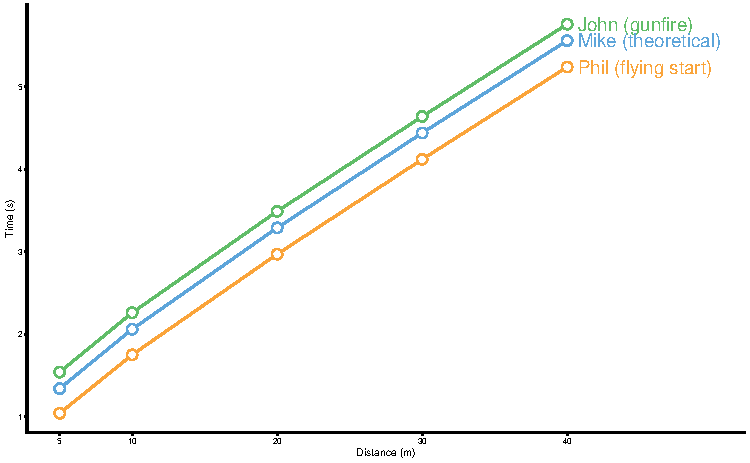
\includegraphics[width=0.9\linewidth]{shorts-simulation-paper_files/figure-latex/mike-phil-john-split-times-1} 

}

\caption{Phil, Mike, and John split times over a 40 \(m\) distance. All three brothers have identical sprint performances but utilize different sprint starts, resulting in different split times.}\label{fig:mike-phil-john-split-times}
\end{figure}

Estimated sprint parameters can be found in Table \ref{tab:mike-phil-john-est-params}. As seen from the results (Table \ref{tab:mike-phil-john-est-params}), estimated short sprint parameters for all three brothers differ from the \emph{true} parameters used to generate the data (i.e., their \emph{true} short sprint characteristics). All three brothers have a bias in estimated parameters due to timing gates' precision to 2 decimals (i.e., 10 \(ms\)). Bias in estimated parameters in Phil's case is due to the flying start involved, while in John's case, it is due to the reaction time involved in the split times.



\begin{table}

\caption{\label{tab:mike-phil-john-est-params}Estimated sprint parameters for Mike, Phil, and John using data from Figure \ref{fig:mike-phil-john-split-times}. All three brothers have identical sprint performance but utilize different sprint starts, which results in different split times, and thus different sprint parameter estimates. Due to the timing gates' precision to 2 decimals (i.e., 10 \(ms\)), estimated Mike's parameters also differ from the \emph{true} values.}
\centering
\begin{tabular}[t]{lrrrr}
\toprule
Athlete & MSS & TAU & MAC & PMAX\\
\midrule
True & 9.00 & 1.12 & 8.00 & 18.0\\
Mike (theoretical) & 9.02 & 1.14 & 7.94 & 17.9\\
Phil (flying start) & 8.60 & 0.61 & 14.00 & 30.1\\
John (gunfire) & 9.59 & 1.62 & 5.93 & 14.2\\
\bottomrule
\end{tabular}
\end{table}

\hypertarget{how-to-overcome-missing-the-initial-force-production-when-using-timing-gates}{%
\subsection{How to overcome missing the initial force production when using timing gates?}\label{how-to-overcome-missing-the-initial-force-production-when-using-timing-gates}}

The literature suggests using a correction factor of +0.5 \(s\) as a viable solution (i.e., simply adding +0.5 \(s\) to split times) to convert to ``first movement'' triggering when utilizing recommended 0.5 \(m\) flying distance behind the initial timing gate (\protect\hyperlink{ref-haugenDifferenceStartImpact2012}{Haugen, Tønnessen \& Seiler, 2012}; \protect\hyperlink{ref-haugenSprintRunningPerformance2016}{Haugen \& Buchheit, 2016}; \protect\hyperlink{ref-haugenSprintMechanicalVariables2019}{Haugen, Breitschädel \& Seiler, 2019}, \protect\hyperlink{ref-haugenSprintMechanicalProperties2020}{2020}). Intriguingly, the average difference between the standing start with a photocell trigger and a block start to gunfire for a 40-meter sprint was 0.27 \(s\) (\protect\hyperlink{ref-haugenDifferenceStartImpact2012}{Haugen, Tønnessen \& Seiler, 2012}). Consequently, although a timing correction factor is required to prevent further inaccuracies in estimates of kinetic variables (e.g., overestimate power), a correction factor that is too big would have the opposite effect (e.g., underestimate power).

\hypertarget{estimated-time-correction-model}{%
\subsubsection{Estimated time correction model}\label{estimated-time-correction-model}}

Instead of using \emph{apriori} time correction from the literature, this parameter may be estimated using the supplied data, together with MSS and TAU. Stenroth, Vartiainen \& Karjalainen (\protect\hyperlink{ref-stenrothForcevelocityProfilingIce2020}{2020}) proposes the same approach, titled the \emph{time shift method}, and the estimated parameter, named the \emph{time shift parameter}. In accordance with the current literature, we have termed this parameter \emph{time correction} (TC) (\protect\hyperlink{ref-vescoviSprintMechanicalCharacteristics2021}{Vescovi \& Jovanović, 2021}).

Using the original equation \eqref{eq:time-distance} to implement the TC parameter now provides the new equation \eqref{eq:time-correction}. Equation \eqref{eq:time-correction} is utilized as the model definition in the \emph{Estimated TC} model, as opposed to the model using equation \eqref{eq:time-distance}, which I have termed \emph{No correction} model. The model in which TC is fixed (i.e., by simply adding TC to split times) is termed the \emph{Fixed TC} model.

\begin{equation}
  t(d) = TAU \times W(-e^{\frac{-d}{MSS \times TAU}} - 1) + \frac{d}{MSS} + TAU - TC \label{eq:time-correction}
\end{equation}

From a regression perspective, the TC parameter can be viewed as an \emph{intercept}. It can be beneficial when we assume a fixed time shift is involved (i.e., reaction time or premature triggering of the timing equipment). If we compare the split times of Mike and John in Figure \ref{fig:mike-phil-john-split-times}, we can notice that the lines are parallel. In this scenario, the \emph{Estimated TC} model can remove bias between Mike and John. The \emph{Estimated TC} model can also help remove bias in estimated parameters in Phil's case. However, if we look closely at Figure \ref{fig:mike-phil-john-split-times}, we will notice that Phil's and Mike's lines are not parallel. This is because there is already some velocity when the initial timing gate is triggered; thus, the time shift is not constant.

These models (i.e., \emph{Fixed TC} of +0.3, +0.5 \(s\), and \emph{Estimate TC} model) are applied to Mike, Phil, and John's split times. The estimated model parameters can be found in Table \ref{tab:all-estimates} and previously estimated parameter values using \emph{No correction} model. As can be noted from Table \ref{tab:all-estimates}, adding +0.3 \(s\) worked well for Phil in terms of approaching \emph{true} parameter values, while adding +0.5 \(s\) was detrimental in un-biasing estimated parameters.

The \emph{Estimated TC} model worked well for all three athletes in terms of un-biasing the parameter estimates. The estimated TC parameter for John was also very close to the \emph{true} reaction time of 0.2 \(s\).

\hypertarget{estimated-flying-distance-model}{%
\subsubsection{Estimated flying distance model}\label{estimated-flying-distance-model}}

Although the \emph{Estimated TC} model performed well in Phil's case (brother doing flying start), instead of assuming time shift (which helps in un-biasing the estimates compared to the \emph{No correction} model), we can utilize model definition that assumes \emph{flying start distance} (FD) involved in the \emph{data-generating-process} (DGP). This \emph{Estimated FD} model utilizes equation \eqref{eq:distance-correction} as the model definition.

\begin{equation}
  \begin{split}
   t(d) &= (TAU \times W(-e^{\frac{-d + FD}{MSS \times TAU}} - 1) + \frac{d + FD}{MSS} + TAU) \\ 
   &\quad-(TAU \times W(-e^{\frac{FD}{MSS \times TAU}} - 1) + \frac{FD}{MSS} + TAU) 
   \end{split}
   \label{eq:distance-correction}
\end{equation}

Table \ref{tab:all-estimates} contains all model estimates for three brothers, including the \emph{Estimated FD} model. We can notice that the \emph{Estimated FD} model unbiased estimates for Phil, but failed to be estimated for John (brother that starts at gunfire and has reaction time involved in his split times). This is because the \emph{Estimated FD} model is \emph{ill-defined} under that scenario and cannot have a \emph{negative} flying distance.

Overall, each model definition has assumed the mechanism of the data generation. \emph{No correction} model assumes perfect synchronization of the sprint initiation with the start of the timing.The \emph{Estimated TC} model introduces a simple intercept that can help estimate parameters when an assumed time shift is involved (e.g., when reaction time is involved or premature triggering of the initial timing gate). \emph{Estimated TC} can also be used when flying start is utilized, but it assumes the constant time shift, which is not the case in that scenario due to already gained velocity at the start. The \emph{Estimated FD} model assumes there is a flying sprint involved in the DGP and, as shown in Table \ref{tab:all-estimates}, can be ill-defined when there is no flying distance involved, but there is a time shift. All three models assume athlete accelerates according to the mono-exponential equation \eqref{eq:velocity-time}.

This work aims to explore the behavior of these three models under simulated and known conditions. This is needed to provide a theoretical understanding of the limits and expected errors of the short sprints modeling, which can later inform more practical studies involving athletes.



\begin{table}

\caption{\label{tab:all-estimates}Estimated sprint parameters for Mike, Phil, and John using data from Figure \ref{fig:mike-phil-john-split-times} using \emph{No correction}, \emph{Fixed time corrections} (TC), \emph{Estimated TC}, and \emph{Estimated FD} models.}
\centering
\begin{tabular}[t]{llrrrrrr}
\toprule
Model & Athlete & MSS & TAU & MAC & PMAX & TC & FD\\
\midrule
True & True & 9.00 & 1.12 & 8.00 & 18.0 &  & \\
\cmidrule{1-8}
 & Mike (theoretical) & 9.02 & 1.14 & 7.94 & 17.9 &  & \\

 & Phil (flying start) & 8.60 & 0.61 & 14.00 & 30.1 &  & \\

\multirow{-3}{*}{\raggedright\arraybackslash No correction} & John (gunfire) & 9.59 & 1.62 & 5.93 & 14.2 &  & \\
\cmidrule{1-8}
 & Mike (theoretical) & 10.01 & 1.93 & 5.19 & 13.0 &  & \\

 & Phil (flying start) & 9.05 & 1.13 & 8.02 & 18.2 &  & \\

\multirow{-3}{*}{\raggedright\arraybackslash Fixed +0.3s TC} & John (gunfire) & 11.29 & 2.79 & 4.05 & 11.4 &  & \\
\cmidrule{1-8}
 & Mike (theoretical) & 11.29 & 2.79 & 4.05 & 11.4 &  & \\

 & Phil (flying start) & 9.62 & 1.61 & 5.98 & 14.4 &  & \\

\multirow{-3}{*}{\raggedright\arraybackslash Fixed +0.5s TC} & John (gunfire) & 13.67 & 4.26 & 3.21 & 11.0 &  & \\
\cmidrule{1-8}
 & Mike (theoretical) & 9.04 & 1.15 & 7.86 & 17.8 & 0.01 & \\

 & Phil (flying start) & 9.00 & 1.08 & 8.35 & 18.8 & 0.28 & \\

\multirow{-3}{*}{\raggedright\arraybackslash Estimated TC} & John (gunfire) & 9.04 & 1.15 & 7.86 & 17.8 & -0.19 & \\
\cmidrule{1-8}
 & Mike (theoretical) & 9.04 & 1.15 & 7.86 & 17.8 &  & 0.00\\

 & Phil (flying start) & 9.03 & 1.16 & 7.82 & 17.7 &  & 0.54\\

\multirow{-3}{*}{\raggedright\arraybackslash Estimated FD} & John (gunfire) &  &  &  &  &  & \\
\bottomrule
\end{tabular}
\end{table}

\hypertarget{methods}{%
\section{Methods}\label{methods}}

\hypertarget{simulation-design}{%
\subsection{Simulation design}\label{simulation-design}}

In this simulation, data is generated using \emph{true} MSS (ranging from 7 to 11 \(ms^-1\), in increments of 0.05 \(ms^-1\), resulting in a total of 81 unique values), MAC (ranging from 7 to 11 \(ms^-2\), in increments of 0.05 \(ms^-2\), resulting in a total of 81 unique values), and flying distance (ranging from 0 to 0.5 \(m\), in increments of 0.01 \(m\), resulting in a total of 51 unique values). Each flying sprint distance consists of 6,561 MSS and MAC combinations.

Splits times are estimated using timing gates positioned at 5, 10, 20, 30, and 40 \(m\), with the rounding to the closest 10 \(ms\). In total, there are 334,611 sprints simulated.

\hypertarget{statistical-analysis}{%
\subsection{Statistical analysis}\label{statistical-analysis}}

MSS, MAC, TAU, and PMAX are estimated for each simulated sprint using \emph{No correction}, \emph{Estimated TC}, and \emph{Estimated FD models}. The agreement between \emph{true} and estimated parameter values is evaluated using the \emph{percent difference} (\(\%Diff\)) estimator (equation \eqref{eq:percent-difference}).

\begin{equation}
  \%Diff = 100 \times \frac{estimated - true}{true}  \label{eq:percent-difference}
\end{equation}

The distribution of the simulated \(\%Diff\) is summarized using \(median\) and 95\% \emph{highest-density continuous interval} (\(HDCI\)) (\protect\hyperlink{ref-kruschkeDoingBayesianData2015}{Kruschke, 2015}, \protect\hyperlink{ref-kruschkeRejectingAcceptingParameter2018}{2018}; \protect\hyperlink{ref-kruschkeBayesianDataAnalysis2018}{Kruschke \& Liddell, 2018a},b; \protect\hyperlink{ref-makowskiBayestestRDescribingEffects2019}{Makowski, Ben-Shachar \& Lüdecke, 2019}).

To provide magnitude interpretation of the \(\%Diff\), \emph{region of practical equivalence} (\(ROPE\)), as well as the proportion of the simulations that lie within \(ROPE\) (\(inside \; ROPE\); expressed as percentage) (\protect\hyperlink{ref-kruschkeDoingBayesianData2015}{Kruschke, 2015}, \protect\hyperlink{ref-kruschkeRejectingAcceptingParameter2018}{2018}; \protect\hyperlink{ref-kruschkeBayesianDataAnalysis2018}{Kruschke \& Liddell, 2018a},b; \protect\hyperlink{ref-makowskiBayestestRDescribingEffects2019}{Makowski, Ben-Shachar \& Lüdecke, 2019}; \protect\hyperlink{ref-jovanovicBmbstatsBootstrapMagnitudebased2020}{Jovanović, 2020}), are calculated. For the purpose of this paper, \(ROPE\) is assumed to be equal to 95\% \(HDCI\) of the \(\%Diff\) using the \emph{No correction} model and no flying distance. Theoretically, \(ROPE\) represents the lowest error (i.e., the best agreement) that can be achieved. It is limited purely by the timing gates measurement precision (i.e., rounding to the closest 10 \(ms\)) and simulated parameters.

In addition to estimating agreement between \emph{true} and estimated parameter values, practitioners are often interested in whether they can use estimated measures to track changes in the \emph{true} measures. A \emph{minimal detectable change} estimator with 95\% confidence (\(\%MDC_{95}\)) (\protect\hyperlink{ref-furlanApplicabilityStandardError2018}{Furlan \& Sterr, 2018}; \protect\hyperlink{ref-jovanovicBmbstatsBootstrapMagnitudebased2020}{Jovanović, 2020}) is utilized to estimate this precision. The \(\%MDC_{95}\) value might be regarded as the minimum amount of change that needs to be observed in the estimated parameter for it to be considered a \emph{true} change.

In this study, \(\%MDC_{95}\) is calculated using \emph{percent residual standard error} (\(\%RSE\); equation \eqref{eq:percent-rse}) of the linear regression between \emph{true} (predictor) and estimated parameter values (outcome) (equation \eqref{eq:smallest-detectable-change}). Since simulated data with the known \emph{true} values are utilized, \(\%RSE\) represents the \emph{percent standard error of the measurement} (\(\%SEM\)) in the estimated parameters.

\begin{equation}
  \%RSE = \sqrt{\frac{\sum_{i=1}^N{(100 \times \frac{y_i - \hat{y_i}}{\hat{y_i}})^2}}{N-2}}  \label{eq:percent-rse}
\end{equation}

\begin{equation}
  \%MDC_{95} = \%RSE \times \sqrt{2} \times 1.96  \label{eq:smallest-detectable-change}
\end{equation}

In addition to providing \(\%MDC_{95}\) for the estimated parameters, the lowest \(\%MDC_{95}\) is estimated using the \emph{No correction} model and no flying distance (\(\%MDC_{95}^{lowest}\)). Theoretically, \(\%MDC_{95}^{lowest}\) represents the lowest \(\%MDC_{95}\) that can be achieved, and it is limited purely by the timing gates measurement precision (i.e., rounding to the closest 10 \(ms\)) and simulated parameters. \(\%MDC_{95}^{lowest}\) is used only as a reference to evaluate estimated parameters' \(\%MDC_{95}\).

The analyses, as mentioned earlier, are performed on both \emph{pooled} dataset (i.e., using all flying distance) and across every flying distance. It is hypothesized that the \emph{Estimated FD} model will have the highest \(inside \; ROPE\) estimates and the lowest \(\%MDC_{95}\) estimates.

Statistical analyses and graph construction were performed using the software R 4.2.1 (\protect\hyperlink{ref-R-base}{R Core Team, 2022}) in RStudio (version 2022.02.3).

\hypertarget{results}{%
\section{Results}\label{results}}

\hypertarget{model-fitting}{%
\subsection{Model fitting}\label{model-fitting}}

Table \ref{tab:tbl-not-fitted} contains failed model fitting for the \emph{Estimated FD} model. These were disregarded from further analysis.

The reason for these failed model fittings is probably in the combination of the very small flying distance and the measurement precision of the timing gates, resulting in ill-defined model that cannot be fitted.



\begin{table}

\caption{\label{tab:tbl-not-fitted}Failed model fittings for the \emph{Estimated FD} model}
\centering
\begin{tabular}[t]{lrrrr}
\toprule
Model & Flying distance (m) & Not fitted & Total & Not fitted (\%)\\
\midrule
Estimated FD & 0.00 & 1765 & 6561 & 26.90\\
Estimated FD & 0.01 & 12 & 6561 & 0.18\\
Estimated FD & 0.02 & 16 & 6561 & 0.24\\
Estimated FD & 0.03 & 10 & 6561 & 0.15\\
Estimated FD & 0.04 & 4 & 6561 & 0.06\\
\addlinespace
Estimated FD & 0.05 & 1 & 6561 & 0.02\\
\bottomrule
\end{tabular}
\end{table}

\hypertarget{percent-difference}{%
\subsection{Percent difference}\label{percent-difference}}

\hypertarget{region-of-practical-equivalence}{%
\subsubsection{Region of practical equivalence}\label{region-of-practical-equivalence}}

Estimated ROPEs are equal to -0.3 to 0.33\% for MSS, -0.73 to 0.74\% for MAC, -1.03 to 1\% for TAU, and -0.5 to 0.5\% for PMAX (Table \ref{tab:tbl-ROPE-pooled} and grey horizontal bars in Figures \ref{fig:graph-ROPE-pooled} and \ref{fig:graph-per-FD}). An interesting finding is that, given simulation parameters (particularly the precision of the timing gates to the closest 10 \(ms\)), MSS has the lowest \(ROPE\) compared to other short sprint parameters. Since \(ROPE\) represents the lowest estimation error, MSS is the parameter that could be, given this theoretical simulation, estimated with the most precision. In contrast, TAU and MAC can be estimated with the least precision.

\hypertarget{pooled-analysis}{%
\subsubsection{Pooled analysis}\label{pooled-analysis}}

The pooled analysis is performed using all flying distances pooled together. As such, the pooled analysis represents the overall estimate of the agreement between \emph{true} and estimated parameter values across simulated conditions.

Figure \ref{fig:graph-ROPE-pooled} depicts the distribution of the pooled \(\%Diff\). As expected, the \emph{Estimated FD} model performed with the highest \(inside \; ROPE\) parameter values (from 20 to 72\%), with the most narrow 95\% \(HDCI\)s (from -5 to 5\%), and no bias involved.

On the other hand, the \emph{No correction} model performed poorly, with the lowest inside \(ROPE\) parameter values (from 2 to 2\%), with the widest 95\% \(HDCI\)s (from -46 to 80\%), and with the apparent bias indicated with the \(median\) parameter values being outside of \(ROPE\) (from -35 to 49\%). In addition, visual inspection of Figure \ref{fig:graph-ROPE-pooled} indicates a \emph{non-normal} distribution of estimated \(\%Diff\) parameter values, demanding further analysis across flying distance values.

The \emph{Estimated TC} model performed similarly to the \emph{Estimated FD} model with slightly lower \(inside \; ROPE\) parameter values (from 9 to 67\%), wider 95\% \(HDCI\)s (from -9 to 8\%), and with obvious bias, although much smaller than the \emph{No correction} model bias (from -3 to 3\%).

Table \ref{tab:tbl-ROPE-pooled} contains the pooled analysis results summary for every model and short sprint parameter.



\begin{figure}

{\centering 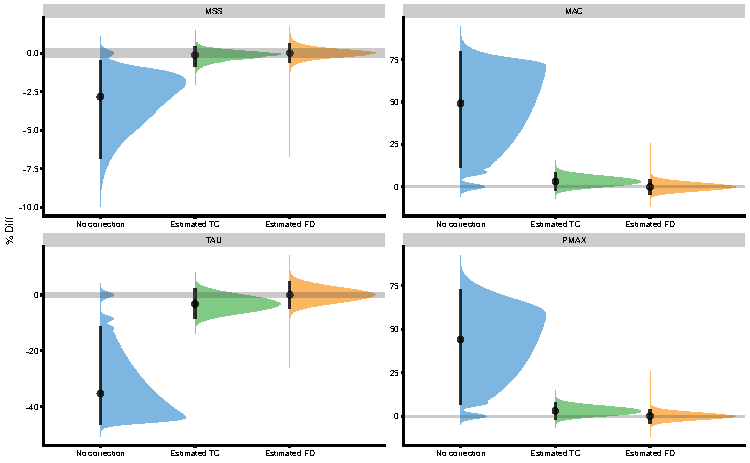
\includegraphics[width=0.9\linewidth]{shorts-simulation-paper_files/figure-latex/graph-ROPE-pooled-1} 

}

\caption{Pooled distribution of the \(\%Diff\). Error bars represent the distribution \(median\) and 95\% \(HDCI\). A grey area represents parameter \(ROPE\) (assumed to be equal to 95\% \(HDCI\) of the \(\%Diff\) using \emph{No correction} model and no flying distance).}\label{fig:graph-ROPE-pooled}
\end{figure}



\begin{table}

\caption{\label{tab:tbl-ROPE-pooled}\(ROPE\)s, a summary of \(\%Diff\) distribution, and \(inside \; ROPE\) for pooled analysis.}
\centering
\begin{tabular}[t]{lrlrr}
\toprule
Parameter & ROPE (\%) & Model & \% Diff & Inside ROPE (\%)\\
\midrule
 &  & No correction & median -3\%, 95\% HDCI [-7 to 0\%] & 2\%\\
\cmidrule{3-5}
 &  & Estimated TC & median 0\%, 95\% HDCI [-1 to 0\%] & 67\%\\
\cmidrule{3-5}
\multirow{-3}{*}{\raggedright\arraybackslash MSS} & \multirow{-3}{*}{\raggedleft\arraybackslash -0.3 to 0.33\%} & Estimated FD & median 0\%, 95\% HDCI [-1 to 1\%] & 72\%\\
\cmidrule{1-5}
 &  & No correction & median 49\%, 95\% HDCI [11 to 80\%] & 2\%\\
\cmidrule{3-5}
 &  & Estimated TC & median 3\%, 95\% HDCI [-2 to 8\%] & 12\%\\
\cmidrule{3-5}
\multirow{-3}{*}{\raggedright\arraybackslash MAC} & \multirow{-3}{*}{\raggedleft\arraybackslash -0.73 to 0.74\%} & Estimated FD & median 0\%, 95\% HDCI [-4 to 4\%] & 25\%\\
\cmidrule{1-5}
 &  & No correction & median -35\%, 95\% HDCI [-46 to -11\%] & 2\%\\
\cmidrule{3-5}
 &  & Estimated TC & median -3\%, 95\% HDCI [-9 to 2\%] & 16\%\\
\cmidrule{3-5}
\multirow{-3}{*}{\raggedright\arraybackslash TAU} & \multirow{-3}{*}{\raggedleft\arraybackslash -1.03 to 1\%} & Estimated FD & median 0\%, 95\% HDCI [-5 to 5\%] & 31\%\\
\cmidrule{1-5}
 &  & No correction & median 44\%, 95\% HDCI [6 to 73\%] & 2\%\\
\cmidrule{3-5}
 &  & Estimated TC & median 3\%, 95\% HDCI [-2 to 8\%] & 9\%\\
\cmidrule{3-5}
\multirow{-3}{*}{\raggedright\arraybackslash PMAX} & \multirow{-3}{*}{\raggedleft\arraybackslash -0.5 to 0.5\%} & Estimated FD & median 0\%, 95\% HDCI [-4 to 4\%] & 20\%\\
\bottomrule
\end{tabular}
\end{table}

\hypertarget{analysis-across-flying-distances}{%
\subsubsection{Analysis across flying distances}\label{analysis-across-flying-distances}}

Figure \ref{fig:graph-per-FD} depicts the esults of the analysis for every flying distance in the simulation. \(inside \; ROPE\) parameter estimates are calculated and depicted in Figure \ref{fig:graph-inside-ROPE} for easier comprehension.

As expected, the \emph{No correction} model demonstrated increasing bias as the flying distance increases (from -46 to 76\%), the widest 95\% \(HDCI\)s (from -47 to 84\%), and the lowest \(inside \; ROPE\) estimated parameter values.

\emph{Estimated TC} showed a small bias trend across flying distances (from -6 to 6\%), resulting in decreasing \(inside \; ROPE\) performance (from 0 to 75\%; see Figure \ref{fig:graph-inside-ROPE}), although with much smaller 95\% \(HDCI\)s (from -10 to 11\%) compared to \emph{No correction} model.

\emph{Estimated FD}, as hypothesized, showed no bias and thus a stable \(inside \; ROPE\) performance across flying distances (see Figure \ref{fig:graph-inside-ROPE}), with minimal 95\% \(HDCI\)s (from -5 to 6\%).



\begin{figure}

{\centering 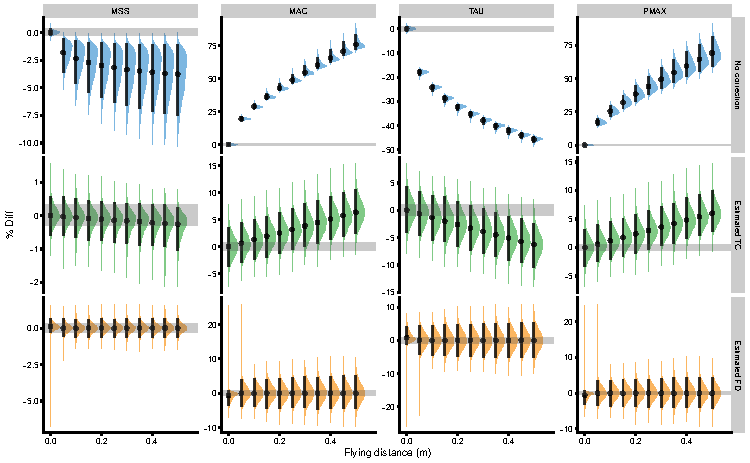
\includegraphics[width=0.9\linewidth]{shorts-simulation-paper_files/figure-latex/graph-per-FD-1} 

}

\caption{Distribution of the \(\%Diff\) across every flying distance in the simulation. Error bars represent the distribution \(median\) and 95\% \(HDCI\). A grey area represents parameter \(ROPE\) (assumed to be equal to 95\% \(HDCI\) of the \(\%Diff\) using \emph{No correction} model and no flying distance). For the less crowded visualization, flying distance in increments of 0.05 \(m\) is plotted.}\label{fig:graph-per-FD}
\end{figure}



\begin{figure}

{\centering 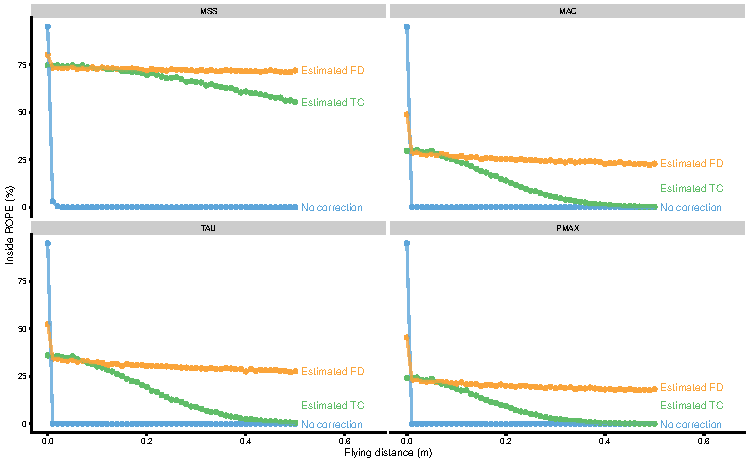
\includegraphics[width=0.9\linewidth]{shorts-simulation-paper_files/figure-latex/graph-inside-ROPE-1} 

}

\caption{\(inside \; ROPE\) estimated across every flying distance in the simulation.}\label{fig:graph-inside-ROPE}
\end{figure}

\hypertarget{minimal-detectable-change}{%
\subsection{Minimal detectable change}\label{minimal-detectable-change}}

\hypertarget{lowest-minimum-detectable-change}{%
\subsubsection{Lowest Minimum Detectable Change}\label{lowest-minimum-detectable-change}}

Estimated \(\%MDCs_{95}^{lowest}\) are equal to 0.45\% for MSS, 1.06\% for MAC, 1.47\% for TAU, and 0.7\% for PMAX (column \emph{lowest} in Table \ref{tab:tbl-pooled-MDC} and dashed grey horizontal lines in Figure \ref{fig:graph-MDC}). An interesting finding is that, given simulation parameters (particularly the precision of the timing gates to the closest 10 \(ms\)), MSS has the lowest \(\%MDCs_{95}^{lowest}\) compared to other short sprint parameters. Since \(\%MDCs_{95}^{lowest}\) represents the lowest minimal detectable change, MSS is the parameter whose change could be, given this theoretical simulation, estimated with the most precision. In contrast, TAU and MAC changes can be estimated with the least precision.

\hypertarget{pooled-analysis-1}{%
\subsubsection{Pooled analysis}\label{pooled-analysis-1}}

Pooled \(\%MDCs_{95}\) represents an estimate of the \emph{sensitivity} to detect \emph{true} change with 95\% confidence when the flying start distance is not standardized (but within simulation parameter limits (ranging from 0 to 0.5 \(m\)). As expected, the \emph{No correction} model demonstrates the highest \(\%MDCs_{95}\) (from 3 to 44\%), while \emph{Estimated TC} and \emph{Estimated FD} demonstrated much smaller \(\%MDCs_{95}\) (from 1 to 8\% and from 1 to 7\%, respectively) (Table \ref{tab:tbl-pooled-MDC}).

An interesting finding is that the MSS parameter showed very low \(\%MDCs_{95}\) across models (from 1 to 3\%), even for the \emph{No correction} model. This indicates that even the non-standardized short sprint monitoring (i.e., without standardized flying distance) using the \emph{No correction} model, given simulation parameters, can be used to track changes in MSS. TAU, MAC, and PMAX parameters, on the other hand, demand much larger \(\%MDCs_{95}\) (from 7 to 44\%, from 6 to 37\%, and from 6 to 36\%, respectively).



\begin{table}

\caption{\label{tab:tbl-pooled-MDC}Pooled \(\%MDCs_{95}\) estimated using pooled simulation dataset.}
\centering
\begin{tabular}[t]{lrrrl}
\toprule
Parameter & lowest & No correction & Estimated TC & Estimated FD\\
\midrule
MSS & 0.45 \% & 3 \% & 1 \% & 1 \%\\
MAC & 1.06 \% & 37 \% & 7 \% & 6 \%\\
TAU & 1.47 \% & 44 \% & 8 \% & 7 \%\\
PMAX & 0.7 \% & 36 \% & 7 \% & 6 \%\\
\bottomrule
\end{tabular}
\end{table}

\hypertarget{analysis-across-flying-distances-1}{%
\subsubsection{Analysis across flying distances}\label{analysis-across-flying-distances-1}}

When estimated across flying distances, \(\%MDCs_{95}\) shows interesting and surprising patterns (Figure \ref{fig:graph-MDC}). For every short sprint parameter, \emph{Estimated TC} showed stable and lower \(\%MDCs_{95}\) compared to \emph{Estimated FD} (from 1 to 6\% and from 1 to 8\%, respectively). This is surprising because even if it has biased estimates of short sprint parameters (see \protect\hyperlink{percent-difference}{Percent difference} results section, mainly Figure \ref{fig:graph-inside-ROPE}) compared to the \emph{Estimated FD}, \emph{Estimated TC} might be more sensitive to detect \emph{changes}, given simulation parameters.

Another surprising finding is that the \emph{No correction} model, even if shown to be highly biased in estimating short sprint parameter values (see \protect\hyperlink{percent-difference}{Percent difference} results section, mainly Figure \ref{fig:graph-per-FD}), showed the lowest \(\%MDCs_{95}\) for the MAC and TAU parameters (from 1 to 5\% and from 1 to 3\% respectively). This indicates that, when short sprint measurement is standardized (i.e., athlete perform with the same flying distance), given the simulation parameters, the \emph{No correction} model can be the most sensitive model to detect \emph{changes} in MAC and TAU parameters. This is the case for the MSS and PMAX parameters (from 0 to 3\% and from 1 to 9\%, respectively).

When it comes to estimating \emph{changes} in short sprint parameters, \emph{change} in MSS is the most sensitive to be detected (from 0 to 3\%) compared to MAC (from 1 to 7\%), TAU (from 1 to 8\%), and PMAX (from 1 to 9\%).



\begin{figure}

{\centering 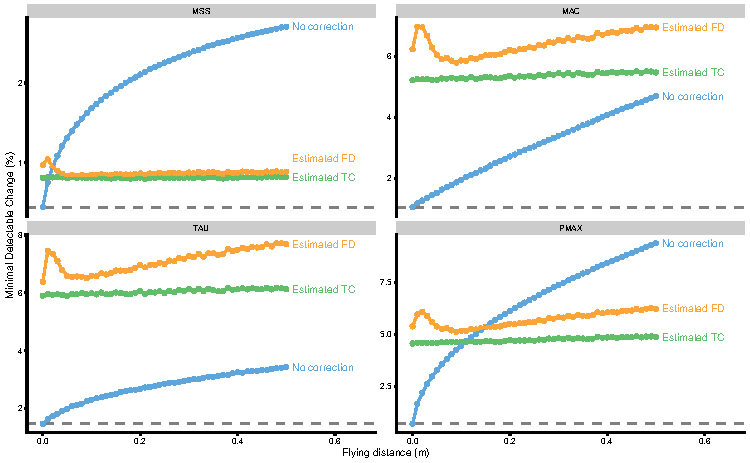
\includegraphics[width=0.9\linewidth]{shorts-simulation-paper_files/figure-latex/graph-MDC-1} 

}

\caption{Estimated \(\%MDCs_{95}\) across every flying distance in the simulation. The dashed line represents \(\%MDCs_{95}^{lowest}\)}\label{fig:graph-MDC}
\end{figure}

\hypertarget{conclusion}{%
\section{Conclusion}\label{conclusion}}

The simulation study employed in this paper demonstrated some expected and unexpected theoretical findings. Among the expected findings are (1) the bias and low \(inside \; ROPE\) performance in estimating short sprint parameters using the \emph{No correction} model, (2) more negligible bias and higher \(inside \; ROPE\) for the \emph{Estimated TC} model, and (3) no bias and highest \(inside \; ROPE\) for the \emph{Estimated FD} model.

The unexpected finding of this study is the performance of the \emph{No correction} model in sensitivity of estimating the \emph{change} of the MAC and TAU parameters, which outperformed the other two models.

When estimating short sprint parameters across models, given simulation parameters, MSS and \emph{change} in MSS can be estimated more precisely compared to TAU, MAC, and PMAX parameters and their \emph{changes}.

In addition to model performances, this simulation study provided the \(ROPE\)s and \(\%MDCs_{95}^{lowest}\). These could be useful for further validity and reliability studies evaluating short sprint model performance involving \emph{real} athletes and timing gates positioned at the same distances with the same rounding.

The take-away message for the practitioners is that besides standardizing the sprint starting technique for the short sprint performance monitoring, it would be wise to utilize and track the results of all three models. The \emph{Estimated FD} model will provide unbiased estimates of the current performance, but the \emph{No correction} model might be more sensitive in detecting changes in TAU and MAC parameters.

This practical conclusion should be taken with caution, since it based on the results of this theoretical simulation. Additional studies involving \emph{real} athletes in evaluating the performance of these three models are needed. These should involve estimating the short sprint parameters agreement between gold-standard (i.e., \emph{criterion}) measure (e.g., radar gun, laser gun, or video analysis) and \emph{practical} timing gates measure. One such study is currently in preparation. In addition to theoretical findings, such a study will provide model performance estimates when biological variability is involved in short sprints, which is not considered in the current study.

\FloatBarrier

\hypertarget{supplemental-material}{%
\section{Supplemental material}\label{supplemental-material}}

The \emph{R Markdown} (\protect\hyperlink{ref-rmarkdown2018}{Xie, Allaire \& Grolemund, 2018}; \protect\hyperlink{ref-rmarkdown2020}{Xie, Dervieux \& Riederer, 2020}; \protect\hyperlink{ref-R-rmarkdown}{Allaire et al., 2022}; \protect\hyperlink{ref-R-bookdown}{Xie, 2022}) source code for this paper and analysis can be found on the GitHub repository: \url{https://github.com/mladenjovanovic/shorts-simulation-paper}.

\hypertarget{references}{%
\section*{References}\label{references}}
\addcontentsline{toc}{section}{References}

\hypertarget{refs}{}
\begin{CSLReferences}{1}{0}
\leavevmode\vadjust pre{\hypertarget{ref-R-rmarkdown}{}}%
Allaire J, Xie Y, McPherson J, Luraschi J, Ushey K, Atkins A, Wickham H, Cheng J, Chang W, Iannone R. 2022. \emph{\href{https://CRAN.R-project.org/package=rmarkdown}{Rmarkdown: Dynamic documents for r}}.

\leavevmode\vadjust pre{\hypertarget{ref-altmannDifferentStartingDistances2015}{}}%
Altmann S, Hoffmann M, Kurz G, Neumann R, Woll A, Haertel S. 2015. Different {Starting Distances Affect} 5-m {Sprint Times}. \emph{Journal of Strength and Conditioning Research} 29:2361--2366. DOI: \href{https://doi.org/10.1519/JSC.0000000000000865}{10.1519/JSC.0000000000000865}.

\leavevmode\vadjust pre{\hypertarget{ref-altmannValiditySingleBeamTiming2017}{}}%
Altmann S, Spielmann M, Engel FA, Neumann R, Ringhof S, Oriwol D, Haertel S. 2017. Validity of {Single}-{Beam Timing Lights} at {Different Heights}. \emph{Journal of Strength and Conditioning Research} 31:1994--1999. DOI: \href{https://doi.org/10.1519/JSC.0000000000001889}{10.1519/JSC.0000000000001889}.

\leavevmode\vadjust pre{\hypertarget{ref-altmannAccuracySingleBeam2018}{}}%
Altmann S, Spielmann M, Engel FA, Ringhof S, Oriwol D, Härtel S, Neumann R. 2018. Accuracy of single beam timing lights for determining velocities in a flying 20-m sprint: {Does} timing light height matter? \emph{Journal of Human Sport and Exercise} 13. DOI: \href{https://doi.org/10.14198/jhse.2018.133.10}{10.14198/jhse.2018.133.10}.

\leavevmode\vadjust pre{\hypertarget{ref-brownAssessmentLinearSprinting2004}{}}%
Brown TD, Vescovi JD, Vanheest JL. 2004. \href{https://www.ncbi.nlm.nih.gov/pmc/articles/PMC3938058}{Assessment of linear sprinting performance: A theoretical paradigm}. \emph{Journal of Sports Science \& Medicine} 3:203--210.

\leavevmode\vadjust pre{\hypertarget{ref-buchheitMechanicalDeterminantsAcceleration2014}{}}%
Buchheit M, Samozino P, Glynn JA, Michael BS, Al Haddad H, Mendez-Villanueva A, Morin JB. 2014. Mechanical determinants of acceleration and maximal sprinting speed in highly trained young soccer players. \emph{Journal of Sports Sciences} 32:1906--1913. DOI: \href{https://doi.org/10.1080/02640414.2014.965191}{10.1080/02640414.2014.965191}.

\leavevmode\vadjust pre{\hypertarget{ref-clarkNFLCombine40Yard2017}{}}%
Clark KP, Rieger RH, Bruno RF, Stearne DJ. 2017. The {NFL Combine} 40-{Yard Dash}: {How Important} is {Maximum Velocity}? \emph{Journal of Strength and Conditioning Research}:1. DOI: \href{https://doi.org/10.1519/JSC.0000000000002081}{10.1519/JSC.0000000000002081}.

\leavevmode\vadjust pre{\hypertarget{ref-edwardsSprintAccelerationCharacteristics2020}{}}%
Edwards T, Piggott B, Banyard HG, Haff GG, Joyce C. 2020. Sprint acceleration characteristics across the {Australian} football participation pathway. \emph{Sports Biomechanics}:1--13. DOI: \href{https://doi.org/10.1080/14763141.2020.1790641}{10.1080/14763141.2020.1790641}.

\leavevmode\vadjust pre{\hypertarget{ref-R-minpack.lm}{}}%
Elzhov TV, Mullen KM, Spiess A-N, Bolker B. 2022. \emph{\href{https://CRAN.R-project.org/package=minpack.lm}{Minpack.lm: R interface to the levenberg-marquardt nonlinear least-squares algorithm found in MINPACK, plus support for bounds}}.

\leavevmode\vadjust pre{\hypertarget{ref-furlanApplicabilityStandardError2018}{}}%
Furlan L, Sterr A. 2018. The {Applicability} of {Standard Error} of {Measurement} and {Minimal Detectable Change} to {Motor Learning Research}---{A Behavioral Study}. \emph{Frontiers in Human Neuroscience} 12:95. DOI: \href{https://doi.org/10.3389/fnhum.2018.00095}{10.3389/fnhum.2018.00095}.

\leavevmode\vadjust pre{\hypertarget{ref-doi:10.1098ux2frspb.1927.0035}{}}%
Furusawa K, Hill AV, Parkinson JL. 1927. The dynamics of "sprint" running. \emph{Proceedings of the Royal Society of London. Series B, Containing Papers of a Biological Character} 102:29--42. DOI: \href{https://doi.org/10.1098/rspb.1927.0035}{10.1098/rspb.1927.0035}.

\leavevmode\vadjust pre{\hypertarget{ref-R-LambertW}{}}%
Goerg GM. 2022. \emph{\href{https://CRAN.R-project.org/package=LambertW}{LambertW: Probabilistic models to analyze and gaussianize heavy-tailed, skewed data}}.

\leavevmode\vadjust pre{\hypertarget{ref-haugenPowerForceVelocityProfilingSprinting2020}{}}%
Haugen TA, Breitschädel F, Samozino P. 2020. Power-{Force}-{Velocity Profiling} of {Sprinting Athletes}: {Methodological} and {Practical Considerations When Using Timing Gates}. \emph{Journal of Strength and Conditioning Research} 34:1769--1773. DOI: \href{https://doi.org/10.1519/JSC.0000000000002890}{10.1519/JSC.0000000000002890}.

\leavevmode\vadjust pre{\hypertarget{ref-haugenSprintMechanicalVariables2019}{}}%
Haugen TA, Breitschädel F, Seiler S. 2019. Sprint mechanical variables in elite athletes: {Are} force-velocity profiles sport specific or individual? \emph{PLOS ONE} 14:e0215551. DOI: \href{https://doi.org/10.1371/journal.pone.0215551}{10.1371/journal.pone.0215551}.

\leavevmode\vadjust pre{\hypertarget{ref-haugenSprintMechanicalProperties2020}{}}%
Haugen TA, Breitschädel F, Seiler S. 2020. Sprint mechanical properties in soccer players according to playing standard, position, age and sex. \emph{Journal of Sports Sciences} 38:1070--1076. DOI: \href{https://doi.org/10.1080/02640414.2020.1741955}{10.1080/02640414.2020.1741955}.

\leavevmode\vadjust pre{\hypertarget{ref-haugenSprintRunningPerformance2016}{}}%
Haugen T, Buchheit M. 2016. Sprint {Running Performance Monitoring}: {Methodological} and {Practical Considerations}. \emph{Sports Medicine} 46:641--656. DOI: \href{https://doi.org/10.1007/s40279-015-0446-0}{10.1007/s40279-015-0446-0}.

\leavevmode\vadjust pre{\hypertarget{ref-haugenDifferenceStartImpact2012}{}}%
Haugen TA, Tønnessen E, Seiler SK. 2012. The {Difference Is} in the {Start}: {Impact} of {Timing} and {Start Procedure} on {Sprint Running Performance}: \emph{Journal of Strength and Conditioning Research} 26:473--479. DOI: \href{https://doi.org/10.1519/JSC.0b013e318226030b}{10.1519/JSC.0b013e318226030b}.

\leavevmode\vadjust pre{\hypertarget{ref-jimenez-reyesRelationshipVerticalHorizontal2018}{}}%
Jiménez-Reyes P, Samozino P, García-Ramos A, Cuadrado-Peñafiel V, Brughelli M, Morin J-B. 2018. Relationship between vertical and horizontal force-velocity-power profiles in various sports and levels of practice. \emph{PeerJ} 6:e5937. DOI: \href{https://doi.org/10.7717/peerj.5937}{10.7717/peerj.5937}.

\leavevmode\vadjust pre{\hypertarget{ref-jovanovicBmbstatsBootstrapMagnitudebased2020}{}}%
Jovanović M. 2020. \emph{Bmbstats: {Bootstrap Magnitude}-based {Statistics} for {Sports Scientists}}. {Mladen Jovanović}.

\leavevmode\vadjust pre{\hypertarget{ref-R-shorts}{}}%
Jovanović M. 2022. \emph{\href{https://mladenjovanovic.github.io/shorts/}{Shorts: Short sprints}}.

\leavevmode\vadjust pre{\hypertarget{ref-jovanovicShortsPackageModeling2020}{}}%
Jovanović M, Vescovi JD. 2020. Shorts: {An R Package} for {Modeling Short Sprints}. \emph{Accepted to International Journal of Strength and Conditioning (IJSC)}.

\leavevmode\vadjust pre{\hypertarget{ref-kruschkeDoingBayesianData2015}{}}%
Kruschke JK. 2015. \emph{Doing {Bayesian} data analysis: A tutorial with {R}, {JAGS}, and {Stan}}. {Boston}: {Academic Press}.

\leavevmode\vadjust pre{\hypertarget{ref-kruschkeRejectingAcceptingParameter2018}{}}%
Kruschke JK. 2018. Rejecting or {Accepting Parameter Values} in {Bayesian Estimation}. \emph{Advances in Methods and Practices in Psychological Science} 1:270--280. DOI: \href{https://doi.org/10.1177/2515245918771304}{10.1177/2515245918771304}.

\leavevmode\vadjust pre{\hypertarget{ref-kruschkeBayesianDataAnalysis2018}{}}%
Kruschke JK, Liddell TM. 2018a. Bayesian data analysis for newcomers. \emph{Psychonomic Bulletin \& Review} 25:155--177. DOI: \href{https://doi.org/10.3758/s13423-017-1272-1}{10.3758/s13423-017-1272-1}.

\leavevmode\vadjust pre{\hypertarget{ref-kruschkeBayesianNewStatistics2018}{}}%
Kruschke JK, Liddell TM. 2018b. The {Bayesian New Statistics}: {Hypothesis} testing, estimation, meta-analysis, and power analysis from a {Bayesian} perspective. \emph{Psychonomic Bulletin \& Review} 25:178--206. DOI: \href{https://doi.org/10.3758/s13423-016-1221-4}{10.3758/s13423-016-1221-4}.

\leavevmode\vadjust pre{\hypertarget{ref-makowskiBayestestRDescribingEffects2019}{}}%
Makowski D, Ben-Shachar M, Lüdecke D. 2019. {bayestestR}: {Describing Effects} and their {Uncertainty}, {Existence} and {Significance} within the {Bayesian Framework}. \emph{Journal of Open Source Software} 4:1541. DOI: \href{https://doi.org/10.21105/joss.01541}{10.21105/joss.01541}.

\leavevmode\vadjust pre{\hypertarget{ref-mangineSpeedForcePower2014}{}}%
Mangine GT, Hoffman JR, Gonzalez AM, Wells AJ, Townsend JR, Jajtner AR, McCormack WP, Robinson EH, Fragala MS, Fukuda DH, Stout JR. 2014. Speed, {Force}, and {Power Values Produced From Nonmotorized Treadmill Test Are Related} to {Sprinting Performance}: \emph{Journal of Strength and Conditioning Research} 28:1812--1819. DOI: \href{https://doi.org/10.1519/JSC.0000000000000316}{10.1519/JSC.0000000000000316}.

\leavevmode\vadjust pre{\hypertarget{ref-marcote-pequenoAssociationForceVelocity2019}{}}%
Marcote-Pequeño R, García-Ramos A, Cuadrado-Peñafiel V, González-Hernández JM, Gómez MÁ, Jiménez-Reyes P. 2019. Association {Between} the {Force}\textendash{{Velocity Profile}} and {Performance Variables Obtained} in {Jumping} and {Sprinting} in {Elite Female Soccer Players}. \emph{International Journal of Sports Physiology and Performance} 14:209--215. DOI: \href{https://doi.org/10.1123/ijspp.2018-0233}{10.1123/ijspp.2018-0233}.

\leavevmode\vadjust pre{\hypertarget{ref-morinSpreadsheetSprintAcceleration2017}{}}%
Morin JB. 2017.A spreadsheet for {Sprint} acceleration {Force}-{Velocity}-{Power} profiling. \emph{Available at} \href{https://jbmorin.net/2017/12/13/a-spreadsheet-for-sprint-acceleration-force-velocity-power-profiling/}{\emph{https://jbmorin.net/2017/12/13/a-spreadsheet-for-sprint-acceleration-force-velocity-power-profiling/}} (accessed October 27, 2020).

\leavevmode\vadjust pre{\hypertarget{ref-morinSpreadsheetSprintAcceleration2019}{}}%
Morin J-B, Samozino P. 2019. Spreadsheet for {Sprint} acceleration force-velocity-power profiling.

\leavevmode\vadjust pre{\hypertarget{ref-morinSimpleMethodComputing2019}{}}%
Morin J-B, Samozino P, Murata M, Cross MR, Nagahara R. 2019. A simple method for computing sprint acceleration kinetics from running velocity data: {Replication} study with improved design. \emph{Journal of Biomechanics} 94:82--87. DOI: \href{https://doi.org/10.1016/j.jbiomech.2019.07.020}{10.1016/j.jbiomech.2019.07.020}.

\leavevmode\vadjust pre{\hypertarget{ref-motulskyIntuitiveBiostatisticsNonmathematical2018}{}}%
Motulsky H. 2018. \emph{Intuitive biostatistics: A nonmathematical guide to statistical thinking}. {New York}: {Oxford University Press}.

\leavevmode\vadjust pre{\hypertarget{ref-R-base}{}}%
R Core Team. 2022. \emph{\href{https://www.R-project.org/}{R: A language and environment for statistical computing}}. Vienna, Austria: R Foundation for Statistical Computing.

\leavevmode\vadjust pre{\hypertarget{ref-samozinoSimpleMethodMeasuring2016}{}}%
Samozino P, Rabita G, Dorel S, Slawinski J, Peyrot N, Saez de Villarreal E, Morin J-B. 2016. A simple method for measuring power, force, velocity properties, and mechanical effectiveness in sprint running: {Simple} method to compute sprint mechanics. \emph{Scandinavian Journal of Medicine \& Science in Sports} 26:648--658. DOI: \href{https://doi.org/10.1111/sms.12490}{10.1111/sms.12490}.

\leavevmode\vadjust pre{\hypertarget{ref-stenrothSpreadsheetSprintAcceleration2020}{}}%
Stenroth L, Vartiainen P. 2020. Spreadsheet for sprint acceleration force-velocity-power profiling with optimization to correct start time. DOI: \href{https://doi.org/10.13140/RG.2.2.12841.83045}{10.13140/RG.2.2.12841.83045}.

\leavevmode\vadjust pre{\hypertarget{ref-stenrothForcevelocityProfilingIce2020}{}}%
Stenroth L, Vartiainen P, Karjalainen PA. 2020. Force-velocity profiling in ice hockey skating: Reliability and validity of a simple, low-cost field method. \emph{Sports Biomechanics}:1--16. DOI: \href{https://doi.org/10.1080/14763141.2020.1770321}{10.1080/14763141.2020.1770321}.

\leavevmode\vadjust pre{\hypertarget{ref-vescoviSprintMechanicalCharacteristics2021}{}}%
Vescovi JD, Jovanović M. 2021. Sprint {Mechanical Characteristics} of {Female Soccer Players}: {A Retrospective Pilot Study} to {Examine} a {Novel Approach} for {Correction} of {Timing Gate Starts}. \emph{Frontiers in Sports and Active Living} 3:629694. DOI: \href{https://doi.org/10.3389/fspor.2021.629694}{10.3389/fspor.2021.629694}.

\leavevmode\vadjust pre{\hypertarget{ref-ward-smithEnergyConversionStrategies2001}{}}%
Ward-Smith AJ. 2001. Energy conversion strategies during 100 m sprinting. \emph{Journal of Sports Sciences} 19:701--710. DOI: \href{https://doi.org/10.1080/02640410152475838}{10.1080/02640410152475838}.

\leavevmode\vadjust pre{\hypertarget{ref-R-bookdown}{}}%
Xie Y. 2022. \emph{\href{https://CRAN.R-project.org/package=bookdown}{Bookdown: Authoring books and technical documents with r markdown}}.

\leavevmode\vadjust pre{\hypertarget{ref-rmarkdown2018}{}}%
Xie Y, Allaire JJ, Grolemund G. 2018. \emph{\href{https://bookdown.org/yihui/rmarkdown}{R markdown: The definitive guide}}. Boca Raton, Florida: Chapman; Hall/CRC.

\leavevmode\vadjust pre{\hypertarget{ref-rmarkdown2020}{}}%
Xie Y, Dervieux C, Riederer E. 2020. \emph{\href{https://bookdown.org/yihui/rmarkdown-cookbook}{R markdown cookbook}}. Boca Raton, Florida: Chapman; Hall/CRC.

\end{CSLReferences}



\end{document}
